%% nicht vergessen draft raus zu nehmen, um echte Bilder einzubinden und die Problem-Vierecke verschwinden zu lassen
\documentclass[11pt,a4paper,oneside,svgnames]{report}

\usepackage[utf8]{inputenc}
\usepackage[T1]{fontenc}
\usepackage{lmodern}
\usepackage{eurosym}
\usepackage[british]{babel}
\usepackage{float}

\usepackage{longtable}
\usepackage{ae}
\usepackage{hyperref}
\usepackage[table]{xcolor}
\usepackage{colortbl}
\usepackage{multirow}
\usepackage{tabularx}
\usepackage{graphicx}
\usepackage{tikz}
\usepackage{kpfonts}
\usepackage[explicit]{titlesec}
\usepackage[acronym,nonumberlist,style=tree]{glossaries}
\usepackage{amssymb}
\usepackage[left=3.65cm,right=3.65cm]{geometry}
\usepackage{listings}


%BEGIN Chapter Definition

\makeatletter
\def\thickhrulefill{\leavevmode \leaders \hrule height 1ex \hfill \kern \z@}
\def\@makechapterhead#1{%
  \vspace*{10\p@}%
  {\parindent \z@ \raggedleft \reset@font
            \scshape \@chapapp{} \thechapter
        \par\nobreak
        \interlinepenalty\@M
    \Huge \bfseries #1\par\nobreak
    %\vspace*{1\p@}%
    \hrulefill
    \par\nobreak
    \vskip 50\p@
  }}
\def\@makeschapterhead#1{%
  \vspace*{10\p@}%
  {\parindent \z@ \raggedleft \reset@font
            \scshape \vphantom{\@chapapp{} \thechapter}
        \par\nobreak
        \interlinepenalty\@M
    \Huge \bfseries #1\par\nobreak
    %\vspace*{1\p@}%
    \hrulefill
    \par\nobreak
    \vskip 50\p@
  }}

%END Chapter Definition

%BEGIN Title Definition

\makeatletter
\def\thickhrulefill{\leavevmode \leaders \hrule height 1pt\hfill \kern \z@}
\renewcommand{\maketitle}{\begin{titlepage}%
    \let\footnotesize\small
    \let\footnoterule\relax
    \parindent \z@
    \reset@font
    \null\vfil
    \begin{flushleft}
      \huge \@title
    \end{flushleft}
    \par
    \hrule height 4pt
    \par
    \begin{flushright}
      \LARGE \@author \par
    \end{flushright}
    \vskip 60\p@
    \vfil\null
  \end{titlepage}%
  \setcounter{footnote}{0}%
}

%END Title Definition

%Verschissener rotierter Text für verschissene Tabelle 14.1/2
\makeatletter
\newsavebox\zzz
\def\mystrut{%
\dimen@\wd\zzz
\divide\dimen@\thr@@
\advance\dimen@-\dp\@arstrutbox
\rule\z@\dimen@}

\def\rotatezzz{%
\rotatebox{90}{\rlap{\kern-\dp\@arstrutbox\usebox\zzz}}}
%END Verschissener rotierter Text

\makeatother
\title{Structured Design for Project ``BookExpress''}
\author{Marc A. Harnos\\ {mharnos@gmail.com} \and Joscha Rapp\\ {jraxxo@gmail.com} \and Christian Schulz\\ {crs.s@gmx.net}}
\author{Marc A. Harnos\\ Joscha Rapp\\ Christian Schulz}
\date{October 2012}



\definecolor{tableHead}{HTML}{40DD0E}
\definecolor{tableEven}{HTML}{D7FCCC}
\definecolor{tableOdd}{HTML}{F0FEEC}
\definecolor{tableFoot}{HTML}{40DD0E}

\definecolor{linkcolour}{rgb}{0,0.2,0.6}

\hypersetup{colorlinks,breaklinks,urlcolor=linkcolour,linkcolor=linkcolour}
\renewcommand{\arraystretch}{1.25}

\makeglossaries

\newglossaryentry{mvc}{name=MVC,description={Model View Controller},plural=MVCs, first={Model View Controller (MVC)}}

\newglossaryentry{jsp}{name=JSP,description={Java Server Page},plural=JSPs, first={Java Server Page (JSP)}, firstplural={Java Server Pages (JSPs)}}

\newglossaryentry{jre}{name=JRE,description={Java Runtime Environment},plural=JRE, first={Java Runtime Environment (JRE)}}

\newglossaryentry{jvm}{name=JVM,description={Java Virtual Machine},plural=JVM, first={Java Virtual Machine (JVM)}}

\newacronym{led}{LED}{light-emitting diode}


\begin{document}

\maketitle
\tableofcontents

\chapter*{Document History}

\begin{center}

\begin{tabular}{|l|l|l|l|}
\hline 
Editor(s) & Date & Purpose of Editing & Version \\ 
\hline 
Harnos, Rapp, Schulz & 2012-10-01 & Initial Document Creation & v0.01 \\ 
\hline
Harnos, Rapp & 2012-10-08 & Fick Das & v0.02 \\ 
\hline
Schulz & 2012-10-08 & Fick Das Nicht - Überstimmt & v0.03 \\ 
\hline 
\end{tabular} 

\end{center}


\chapter{Introduction}
This structured design gives a detailed overview of the software design and system architecture, based on the previously developed requirement analysis and structured analysis. The structured design should be later on used for the implementation of the "BookExpress" system.

This document describes the specifications for the software architecture, the functional abstraction layer of the previously defined data flow diagrams and detailed specification of the system modules.

The description of the specific modules will vary in abstraction, allowing the software architect to implement his own, or the companies preferred, standards, without interfering in product functionality; whenever necessary the definitions provided will be more granular ensuring consistent quality and enforcing expected behaviour.

Some description will have overlapping information with the requirements specification, in case this document is sent stand alone, to assure all information is being provided.

\chapter{Environment / General~Architecture}
This chapter describes the general architecture of the system and the environment, general information will be provided for the system here, which will be described in the next chapter in depth; also detailed hardware and software specifications will be discussed in this chapter.

\begin{figure}[H]
 \begin{center}
  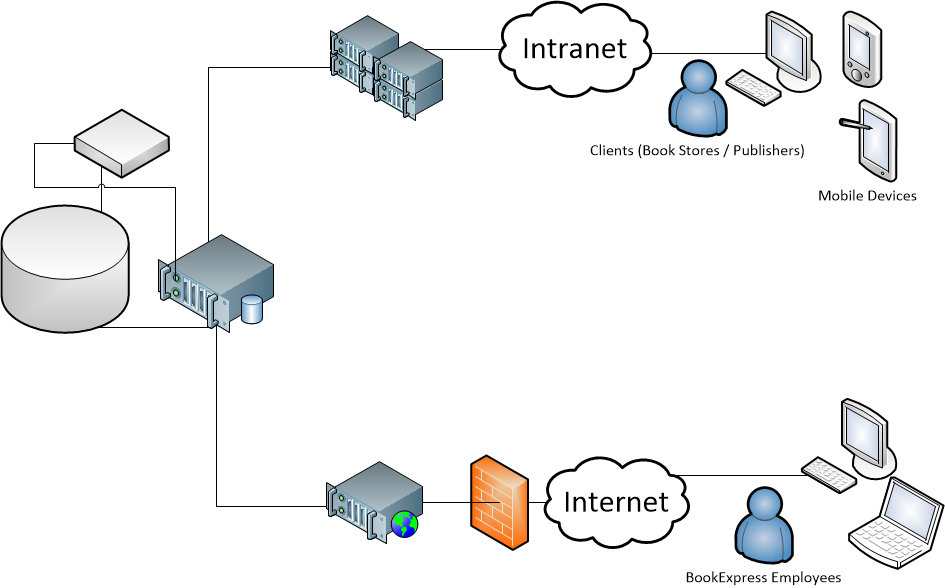
\includegraphics[width=\textwidth]{Hardware Structure.png}
 \end{center}
 \caption{Hardware Structure}
\end{figure}

\section{Application Server}
The application server incorporates the business logic and database requests and queries. It provides the business and data access layer of the application which is described in \ref{sec:mvc-pattern}. The application server processes requests from the web server and makes data objects in response to those requests, which can be used by the web server.

\section{Web Server}
The web server is implemented as a separate Java web server, like Tomcat, which can be incorporated in the application server, but also can run stand alone on another server. The server only processes requests from the web interface and decides which page to show, or if data received can be stored.

The web server is only accessible through a certain range of ports which are necessary to display standard web pages and secure web pages, to prevent hijacking or the manipulation of server configuration files.

\section{Database Server}
The database server provides any data requested from the application server and can be hosted on separate servers, but could also be on the same hardware infrastructure. The server should be an advanced and stable system like an IBM DB2 System or an Oracle Database Management System, a MySql solution might also be applicable, but the better performance, faster response times and stability of dedicated database systems would be preferable.

\section{Server Environment}
For the product to work, servers must be able to run the \gls{jvm} on which our Java application server runs. The server could be any type of mainframe with virtualisation technology; but also any type of individual Unix or Windows servers with the server applications physically separate.

An Unix system is preferable for the fewer system load from the operating system and improved stability. The data storage could also be allocated on separate storage units like medium sized magnetic storage units from IBM or HP.

The important part is, that the servers have at least this kind of specification for the individual servers, the application server, web server and database server, or cumulative on big servers or mainframes:

\begin{itemize}
	\item at least 4GHz Quad-Core CPU per server
	\item for each server at least 12 GB of RAM, for the database server at least 32GB
	\item enough storage for temporary files and data, at least 1-3 TB per server, and at least 3-5TB for the application server
\end{itemize}

A fast LAN connection is required for each server; this connection should at least be a 10GBit connection so servers in a server farm or computing centre communicate as fast as possible minimizing data retrieval times.

\section{Client Environment}
\subsection{Hardware}
The hardware specifications for the client are basically the minimal requirements of the operating system. The client also should not have less than 2GB of RAM.

Also the machine has to be able to access the network via an ethernet adapter so information from the web server application can be retrieved. The client's machine has to have enough free usb ports to support additional hardware like the graphical tablet, bar code readers and other possible hardware additions to the stand alone client.
\subsection{Software}
\subsubsection{Web Interface}
The web interface is accessed through a web browser - this browser should be standards compliant.

This list shows the supported browsers, but any other browser can work too, as long as it implements standards obedient rendering engines.

\begin{itemize}
	\item Firefox (version 3.5 or higher)
	\item Chrome (any version)
	\item Safari (version 4 or higher)
	\item Opera (version 9 or higher)
	\item Internet Explorer (version 10 or higher)
\end{itemize}
\subsubsection{Client Application}
The client application for "BookExpress" employees should have the \gls{jre} installed, so the application can be executed. The operating system does not matter, but some hardware could possibly not be accessed by certain operating system, therefore also drivers for special hardware add ons, like the previously mentioned tablets and bar code readers, should be installable and present.

\chapter{Software Architecture}
The software architecture of a system is the set of structures needed to reason about the system, which comprise software elements, relations among them, and properties of both. The term also refers to documentation of a system's "software architecture".\footnote{ Clements, Paul; Felix Bachmann, Len Bass, David Garlan, James Ivers, Reed Little, Paulo Merson, Robert Nord, Judith Stafford (2010). Documenting Software Architectures: Views and Beyond, Second Edition. Boston: Addison-Wesley. ISBN 0-321-55268-7.}\footnote{Bass, Len; Paul Clements, Rick Kazman (2012). Software Architecture In Practice, Third Edition. Boston: Addison-Wesley. pp. 25–37. ISBN 0-321-81573-4.}

In this chapter the programming pattern which the software architect has to implement is discussed at first, then common techniques for standardizing the code and enhancing readability and the used software and at last the implementation of the pattern into the software solution itself.

\section{Programming Pattern}
\label{sec:mvc-pattern}
The "BookExpress" software should implement a simple \gls{mvc} pattern separating the user visible output from the internal data processing structures much like CSS separates the styling of a webpage from the HTML markup.

The "Model" part of this set up fetches data from databases and holds them in objects - it is essentially the "data storage" of the application. The controller and view must not make any database queries, all data required for the specific controller/view has to be provided by the model itself, which in turn does make the necessary database requests. This can speed up the data retrieving process with smart caching times on the model part and also ensures a higher level of security by minimizing the chance of SQL-Injections possibly performed on the controller/view.

The "View" is essentially anything the user gets to see on his side of the application - the user interface. It also is the only point where the user can interact with the application, evaluating and providing data. The view itself can only retrieve data from the model, it can never make direct database lookups.

The "Controller" holds the business and processing logic of the software. It decides which view should be displayed to the user and which model could be used. Any data sent from the view/the user is processed by the controller and sent to the appropriate models.

In the "BookExpress" software there are two different implementations of this \gls{mvc} pattern. The web interface is the view component for the book shops and publishers, they interact with this view over their web browsers.
For this view, the controller is implemented on the application server as a web server, providing requested views and processing delivered input data. The communication between the view and controller is made over the standard network protocol tcp/ip and the data transmitted varies from standard HTML/text pages to compressed JSON data, for asynchronous and dynamic client view updates.

The "Model" in the first - and also in the second - set up is the application server itself, on which the web server runs. The application server is on the same machine as the web server, but logically a separate entity; it has access to the database server, which can also run on the same hardware, but also could run on a different machine. The data transmitted from model to controller and vice versa is composed of data objects transmitted binary for instant usage on the individual server; we do not have to compress data here, or serialize it, for the lack of data travelling distance.

In the second case, when the "BookExpress" employees use the client application software, the \gls{mvc} varies a bit from the web interface implementation. Here the application itself has its separate model, view and controller, which in turn all three act as a controller \textbf{and} view unit and the outlying model is on the application server in an different location. Therefore the data transmitted from this controller construct to the model and vice versa has to be compressed and serialized, utilizing JSON and gzip compression to accomplish fast serialisation and minimisation for faster response times and as little as possible data transferred. The communication between the inner model and inner controller are - as with the implementation on the application server - uncompressed and binary transferrals of Java objects.

This set up accomplishes that the inner model can cache data and minimize the needed look up to the model on the application server, where as the inner controller and view do not have to be modified for this "special environment"; they get their data as if they were directly connected to the outer model - but with enhanced performance.

\begin{figure}[H]
 \begin{center}
  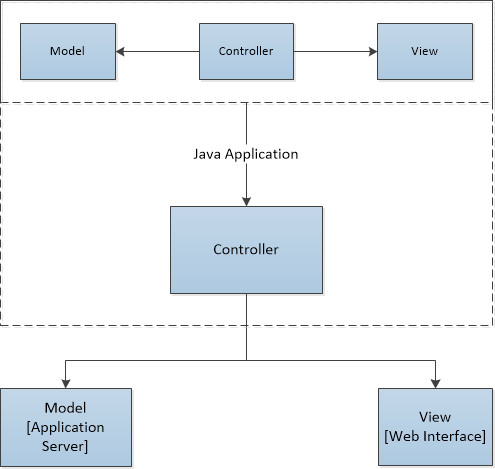
\includegraphics[width=\textwidth]{MVC-small.png}
 \end{center}
 \caption{MVC Pattern}
\end{figure}

\section{Programming Techniques and Software}
For standardisations and readabilities sake simple rules should be honoured to ensure a consistent look of program code, making it for new software architects joining the team easier to understand the code and find code parts faster. Those rules are arbitrary and should be agreed upon the development team; they should be defined at the beginning of the project and extended if necessary. An example for such a rule would be the placement of curly braces after method declarations, they could be defined directly after the declaration or in a new line.

\lstset{
	tabsize=4,
	rulecolor=,
	language=Java,
        basicstyle=\scriptsize,
        upquote=true,
        aboveskip={1.5\baselineskip},
        columns=fixed,
        showstringspaces=false,
        extendedchars=true,
        breaklines=true,
        prebreak = \raisebox{0ex}[0ex][0ex]{\ensuremath{\hookleftarrow}},
        frame=single,
        showtabs=false,
        showspaces=false,
        showstringspaces=false,
        identifierstyle=\ttfamily,
        keywordstyle=\color[rgb]{0,0,1},
        commentstyle=\color[rgb]{0.133,0.545,0.133},
        stringstyle=\color[rgb]{0.627,0.126,0.941},
        captionpos=b
}

\begin{lstlisting}[caption={Example of method declaration with curly braces in single and new line},label=javaCodeExampleCurlyBraces]
/*
 * Example for main method with curly braces directly 
 * after method declaration
 */
public static void main(String[] argv) {
	String where = "down below";
	System.out.println("Your code goes " + where);
}

/*
 * This main method declaration has the curly braces 
 * after a line break
 */
public static void main(String[] args)
{
	System.out.println("Your code goes here, maybe.");
}
\end{lstlisting}

The application server should be implemented with a Java application server; it does not matter if this server application is commercial or open source, as long as it is Sun/Oracle certified for Java EE application servers\footnote{http://www.oracle.com/technetwork/java/javaee/overview/compatibility-jsp-136984.html}.
The server could be a WebSphere Application Server from IBM, but also an TomEE from Apache, as long as it has all the required server modules for running a web server.

Java EE should be used due to a number of advantages:
\begin{itemize}
	\item Implementation of MVC pattern comes naturally with Java EE application servers, because of how Java in general works and in particular the application server is modelled with APIs and object oriented modularisation
	\item It is a very popular software used by many companies, so the chances that the implementing software architect has already experience with it is very likely
	\item The web server system is faster than common PHP servers, due to the compilation of web pages rather than script interpretation
\end{itemize}

For the database there is also the choice between a proprietary, commercial system like DB2 from IBM or an open source solution like a MySQL server; the important thing is, that the database supports standard SQL queries - not requiring the alteration of SQL statements/queries for the sake of proprietary solutions like special JOIN cases on some Microsoft database systems.

\section{Implementation}
\subsection{Data Storage/Application Server (Model)}
The model, which runs on the Java application server, has a intermediate connection to the database server and delivers the required information for the view and controller in form of Java Beans or JSON strings.

The model also has an implemented security layer, denying access to data, which the user has no privileges to and blocking malicious requests. This security layer has to work quick, and in general the model has to be very responsive, due to the high data load.

\subsection{Web Interface (View)}
The view is the point, the interaction between the book stores, publishers and the system takes place. The web interface should look the same on, and work with any new and standards compliant web browser; the supported browsers should at least include Mozilla Firefox from version 3.5 onwards, Chrome, Opera from version 9 onwards, Safari, and Internet Explorer from version 10 onwards.

The view itself should output standard complaint HTML5 code, and use modern JavaScript libraries to enhance the user experience and make user work flow easier to understand, i.e. by implementing visual clues which data is currently missing and suggesting search and input terms where appropriate.

The work flow has to be easy to understand, and the input fields and buttons should be recognised fast and placed on similar locations for each individual task, for faster learning curves and easy and fast pattern remembering.

\subsection{Application Server/Web Server (Controller)}
The controller is processing user data, which always implies input errors and the possibility of an attack to the system. The data has to be checked for any inconsistency regarding data type and for missing data - also any attempt of system intrusion has to be recognised and prevented.
The controller has a security and rights management layer implemented, preventing users from seeing views, they should not be able to see.

The controller is running on a web server and is realised through \glspl{jsp}.

\subsection{Client Application (Controller/View)}
The client application is a stand alone Java application which incorporates the model, view and controller into one program, and is regarded as a controller unit itself. The data is retrieved from the application server and transmitted serialised through JSON strings into the model of the application. Hereby security is very important, the data is never transmitted without encryption ensuring packages could not be sniffed over the network. The whole application as a controller has to be written so it cannot be manipulated in a form, where the user is given more rights than he actually has - without model authorisation the controller should not be able to process any data to the view nor retrieve such data from the model on the web server itself.

The client application should be very responsive and fast - it also should integrate in the system very well enabling features as drag\&drop and the support for specialised hardware like graphical tablets for signature processing and bar code readers or gps tracking devices.

\section{Model Layers}
\begin{figure}[H]
 \begin{center}
  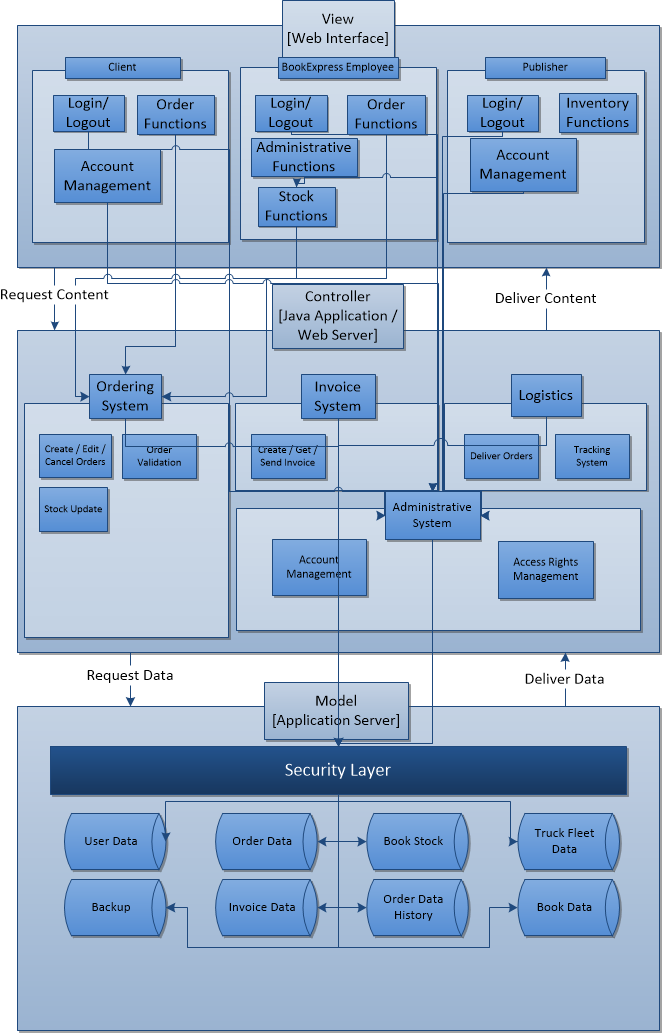
\includegraphics[width=\textwidth]{LayeredModel.png}
 \end{center}
 \caption{Model Layers}
\end{figure}

\section{Module Relations/Dependencies}
This section shows the relations and dependencies between the modules in a layer structure, showing relations between the X big modules, A, B C, and listing their sub modules accordingly.

TODO: insert image showing relations [ref: T3 Model p9]

\chapter{Software Modules}


\chapter{Data Dictionary}

\section{User Data}

\begin{longtable}{p{3.5cm}p{0.5cm}p{8.5cm}}
Client File & = & \{Client Data\} \\
\\
Client Data & = & Client PIN\\
&  & + Address\\
&  & + Correspondent\\
&  & + Contract Data\\
&  & + \{Order\}\\
&  & + \{Invoice\}\\
&  & + (Sales Volume)\\
&  & + Login Data \\
& = & Publisher Data\\
& = & Book Store Data\\
\\
Address & = & [Street + Street Number $|$ Post-Office Box]\\
&  & + Name\\
&  & +  (Country Symbol)\\
&  & +  Postal Code\\
&  & + City\\
&  & + Phone Number\\
&  & + (Fax)\\
&  & + Email Address\\
\\
Name & = & Form Of Address\\
&  & + (Title)\\
&  & + Forename\\
&  & + Surname\\
&  & + (Trade Name)\\
& = & Author\\
& = & Publisher\\
& = & Driver\\
\\
Login Data & = & [Client PIN $|$ Employee PIN]\\
&  & + Password \\
\\
Correspondent & = & Name\\
&  & + (Email)\\
\end{longtable}


\section{Order Data}

\begin{longtable}{p{3.5cm}p{0.5cm}p{8.5cm}}
Order & = & Order Data\\
\\
Order Data & = & Order PIN\\
&  & + 1\{Article\}\\
&  & + Order Status\\
&  & + Date \\
\\
Order Status & = & [Processing $|$ Valid $|$ Invalid $|$ Logistics $|$ Delivery $|$ Delivered $|$ Canceled] \\
\\
Date & = & Hour\\
&  & + Minute\\
&  & + Day\\
&  & + Month\\
&  & + Year\\
\end{longtable}

\section{Internal Data}

\subsection{Book Stock}
\begin{longtable}{p{3.5cm}p{0.5cm}p{8.5cm}}
Stock & = & \{Article\} \\
\\
Article & = & Book Data\\
&  & + Amount\\
\\
Book Data & = & [ISBN $|$ UPC $|$ EAN]\\
&  & + 1\{Author\}\\
&  & + Title\\
&  & + Publisher\\
&  & + (Article Cover)\\
&  & + Price\\
&  & + Availability\\
\\
Availability & = & [In Stock $|$ Ordered at Publisher $|$ N/A]\\
\end{longtable}

\subsection{Truck Information}

\begin{longtable}{p{3.5cm}p{0.5cm}p{8.5cm}}
Truck Fleet Data & = & Driver\\
&  & + Registration Number\\
&  & + Truck Status \\
\\
Truck Status & = & [Boxing $|$ Parcel Sorting Centre $|$ Delivering $|$ Traffic Jam $|$ Delivered] \\
\end{longtable}

\subsection{User Data}
\begin{longtable}{p{3.5cm}p{0.5cm}p{8.5cm}}
Contract Data & = & Contract PIN\\
& & + Signing Date\\
& & + [Client Data $|$ Employee Data]\\
& & + File On Server\\
\\
Signing Date & = & Day\\
&  & + Month\\
&  & + Year\\
\\
Invoice & = & Client Data\\
&  & + Order\\
&  & + Invoice PIN\\
&  & + Invoice Status\\
\\
Invoice Status & = & [Paid $|$ Open]\\
\end{longtable}

\subsection{Employee}

\begin{longtable}{p{3.5cm}p{0.5cm}p{8.5cm}}
Employee File & = & \{Employee Data\}\\
\\
Employee Data & = & Employee PIN\\
&  & + Address\\
&  & + Contract Data\\
&  & + Login Data\\
&  & + Administrator\\
\\
Administrator & = & [True $|$ False]
\end{longtable}


\chapter{Appendices}
\addcontentsline{toc}{section}{Glossary}
\addcontentsline{toc}{section}{Acronyms}
\printglossaries

\end{document}